\section{Refactoring}
\noindent Le refactoring est une fonctionnalité qui permet de modifier le code de manière automatique comme par exemple renommer une variable, une méthode, etc.
C'est une fonctionnalité très appréciée des développeurs car elle permet de gagner du temps et d'éviter les erreurs de frappe ou simplement les oublis lors de la modification du code.
\newdoubleline
Dans notre cas, seul la partie renommage d'un prédicat, d'un atome ou d'une variable nous intéresse.
En effet, il est fréquent de renommer un prédicat ou une variable dans un fichier Prolog et il est important de renommer
toutes les occurrences de ce prédicat ou de cette variable dans tous les fichiers inclus.

\subsection{Renommer un prédicat}
\noindent Pour renommer un prédicat, il faut d'abord récupérer le prédicat à renommer.
Ensuite, il faut récupérer tous les fichiers inclus dans le fichier courant ainsi que tous les fichiers inclus dans ces
fichiers inclus et ainsi de suite.
\newdoubleline
Il faut ensuite remplacer toutes les occurrences du prédicat par le nouveau nom.
\newdoubleline Exemple d'un renommage de prédicat:

\begin{figure}[H]
    \centering
    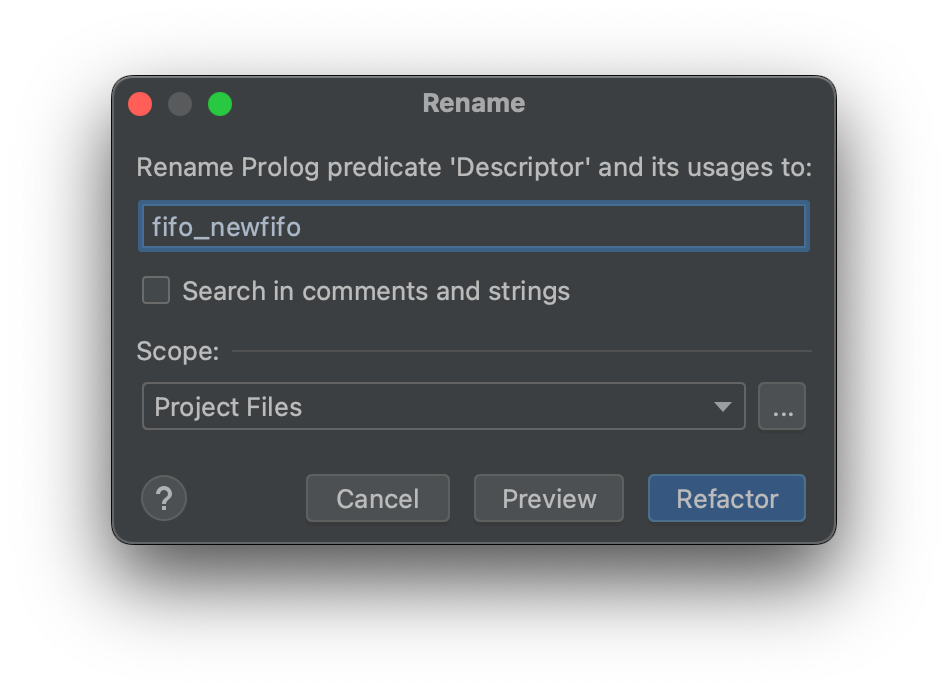
\includegraphics[width=0.8\textwidth]{images/Refactor_window.png}
    \caption{Fenêtre de renommage d'un prédicat}
    \label{fig:refactor_window}
\end{figure}

\begin{figure}[H]
    \centering
    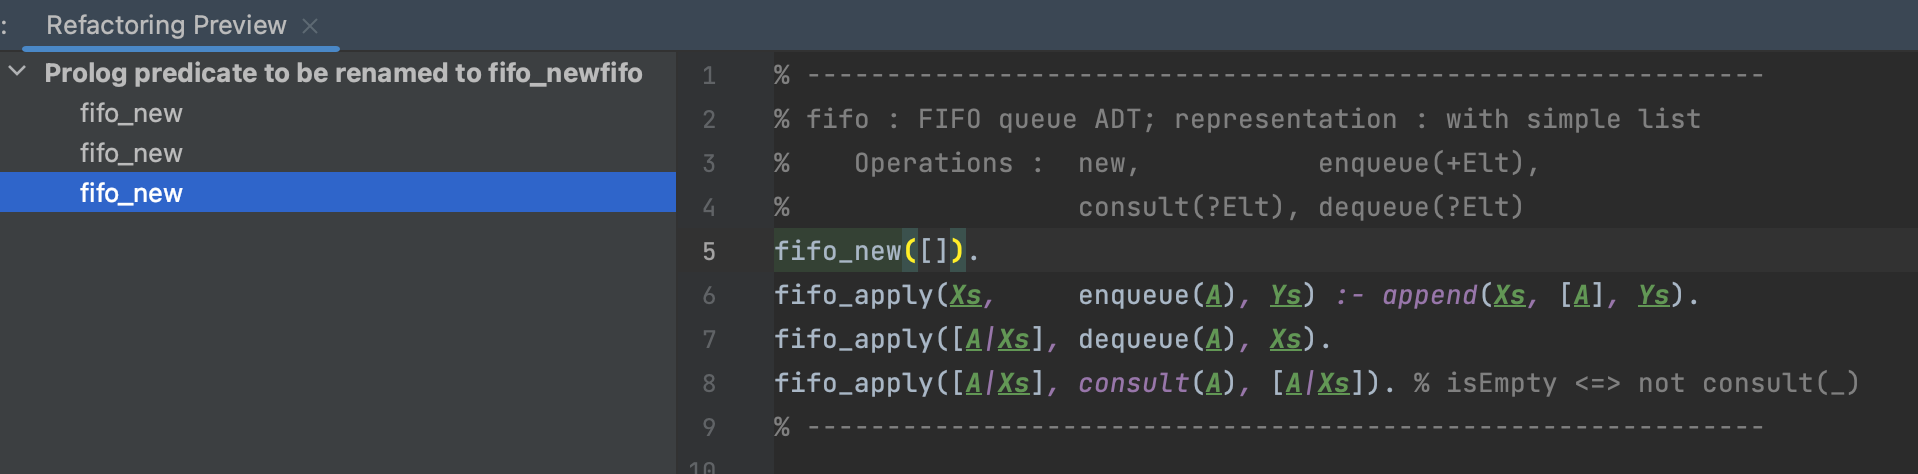
\includegraphics[width=0.8\textwidth]{images/Refactoring_preview.png}
    \caption{Aperçu du refactoring}
    \label{fig:refactor_preview}
\end{figure}

\subsection{Renommer une variable}
\noindent Pour ce qui est du renommage d'une variable, la portée du refactoring est limitée à la phrase Prolog dans laquelle se trouve la variable.
\newdoubleline
Le fonctionnement est similaire à celui du renommage d'un prédicat, à la différence que l'on ne va pas chercher en dehors de la phrase Prolog dans laquelle se trouve la variable.

\subsection{Fonctionnement du renommage}
\noindent Le fonctionnement du renommage est le suivant:
\begin{enumerate}
    \item On récupère le prédicat ou la variable à renommer.
    \item On récupère tous les fichiers inclus dans le fichier courant.
    \item On récupère tous les fichiers inclus dans ces fichiers inclus et ainsi de suite.
    \item On affiche un aperçu des modifications.
    \item On remplace toutes les occurrences du prédicat ou de la variable par le nouveau nom.
\end{enumerate}

\noindent La classe qui gère le renommage est \textbf{PrologRenamePsiElementProcessor}.
Voici une brève description des méthodes de cette classe héritée de \textbf{RenamePsiElementProcessor}:
\begin{enumerate}
    \item \textbf{canProcessElement}: Cette méthode permet de vérifier si l'élément peut être renommé. Dans notre cas, on vérifie si l'élément est un prédicat ou une variable.
    \item \textbf{prepareRenaming}: Cette méthode permet de préparer le renommage. Dans notre cas, on récupère tous les prédicats de tous les fichiers touchés par le renommage.
    \item \textbf{renameElement}: Cette méthode permet de renommer chaque prédicat/variable.
\end{enumerate}